%% Beispiel-Präsentation mit LaTeX Beamer im KIT-Design
%% entsprechend den Gestaltungsrichtlinien vom 1. August 2020
%%
%% Siehe https://sdqweb.ipd.kit.edu/wiki/Dokumentvorlagen

%% Beispiel-Präsentation
\documentclass{sdqbeamer} 
 \usepackage{xcolor}
%% Titelbild
\titleimage{banner_2020_kit}

%% Gruppenlogo
\grouplogo{} 

%% Gruppenname
%\groupname{Institut für Informationssicherheit und Verlässlichkeit (KASTEL)}

% Beginn der Präsentation

\title[Refaktorisierung einer Architekturanalyse für Vertraulichkeit]{Refaktorisierung einer Architekturanalyse für Vertraulichkeit}
\subtitle{Praktikum Ingeneursgemäße Softwareentwicklung} 
\author[Alina Valta]{Alina Valta}

\date[10.\,03.\,2022]{10. März 2022}

% Literatur 
 
\usepackage[citestyle=authoryear,bibstyle=numeric,hyperref,backend=biber]{biblatex}
\addbibresource{presentation.bib}
\bibhang1em

\begin{document}

%Titelseite
\KITtitleframe

%Inhaltsverzeichnis
\begin{frame}{Inhaltsverzeichnis}
\tableofcontents
\end{frame}

\section{Vertraulichkeitsanaylse}
\begin{frame}{Vertraulichkeitsanayse}
\begin{columns}[c]
	\column{.25\textwidth}
	\centering
	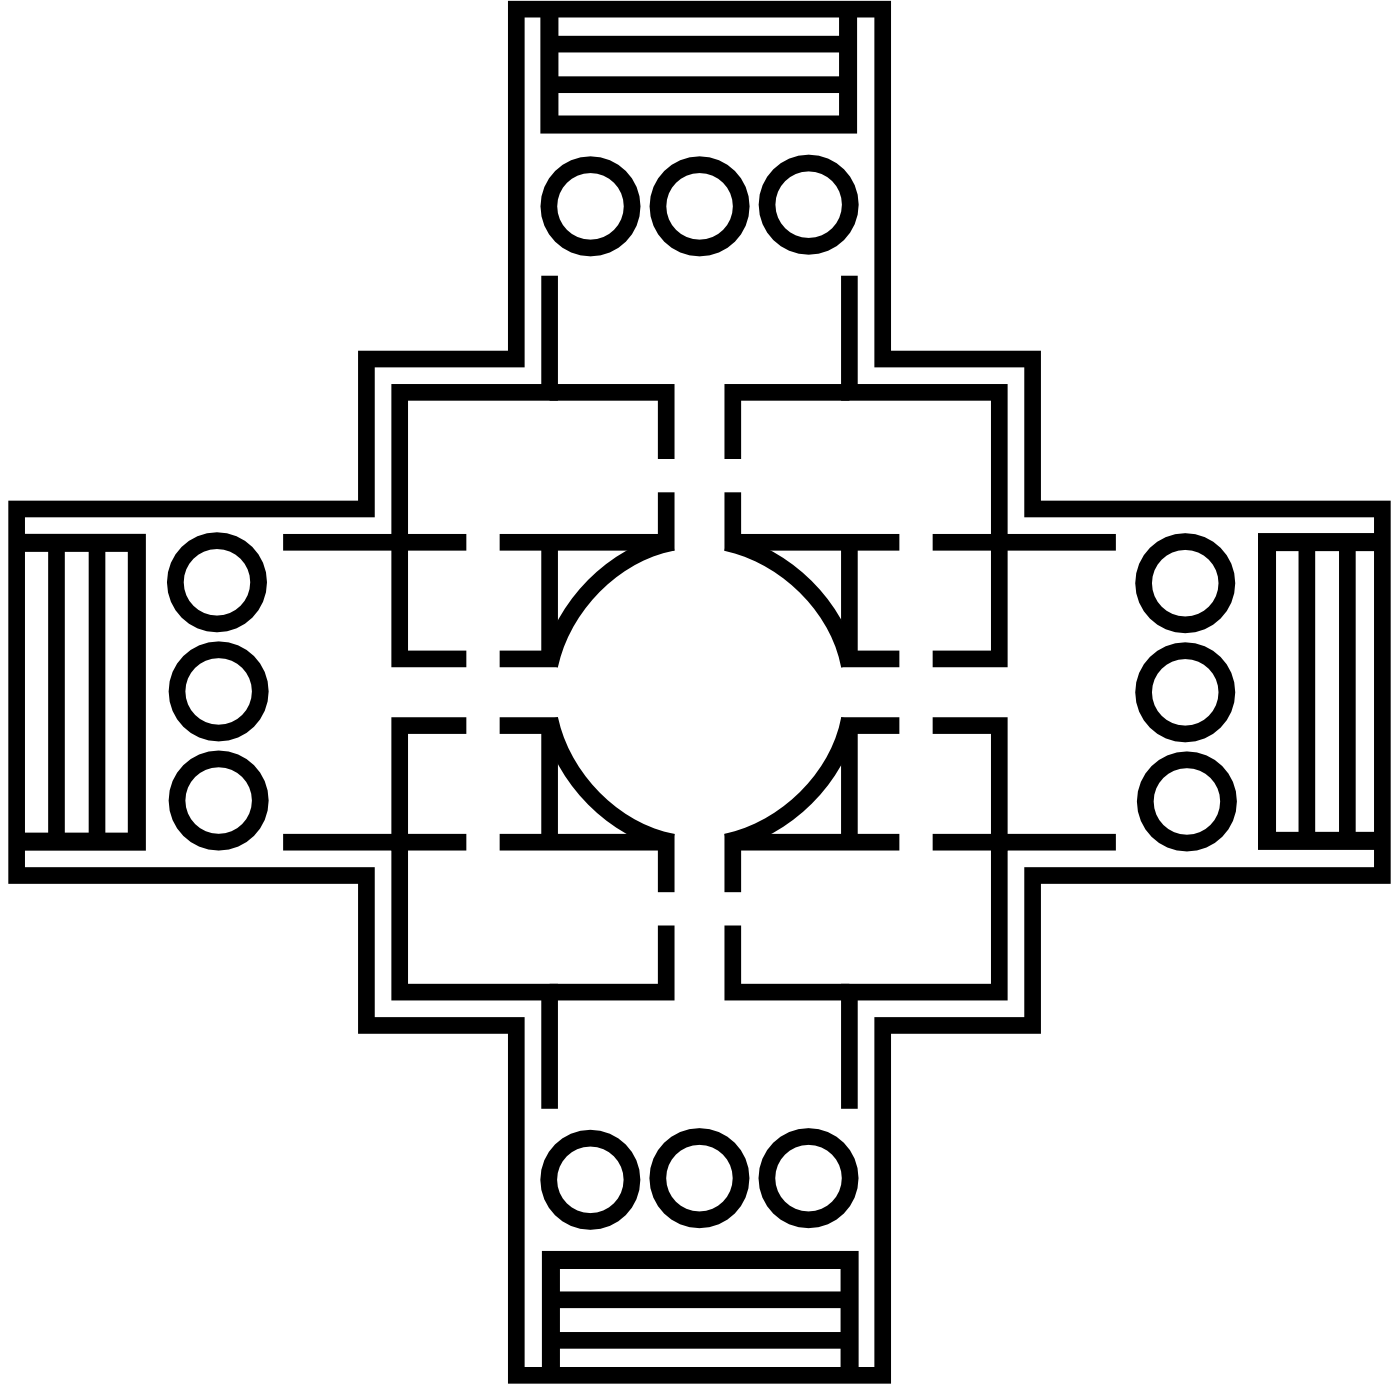
\includegraphics[width=0.6\textwidth]{images/Palladio-logo.png}
	\vspace{0.05\textheight}
	\column{.25\textwidth}
	\centering
	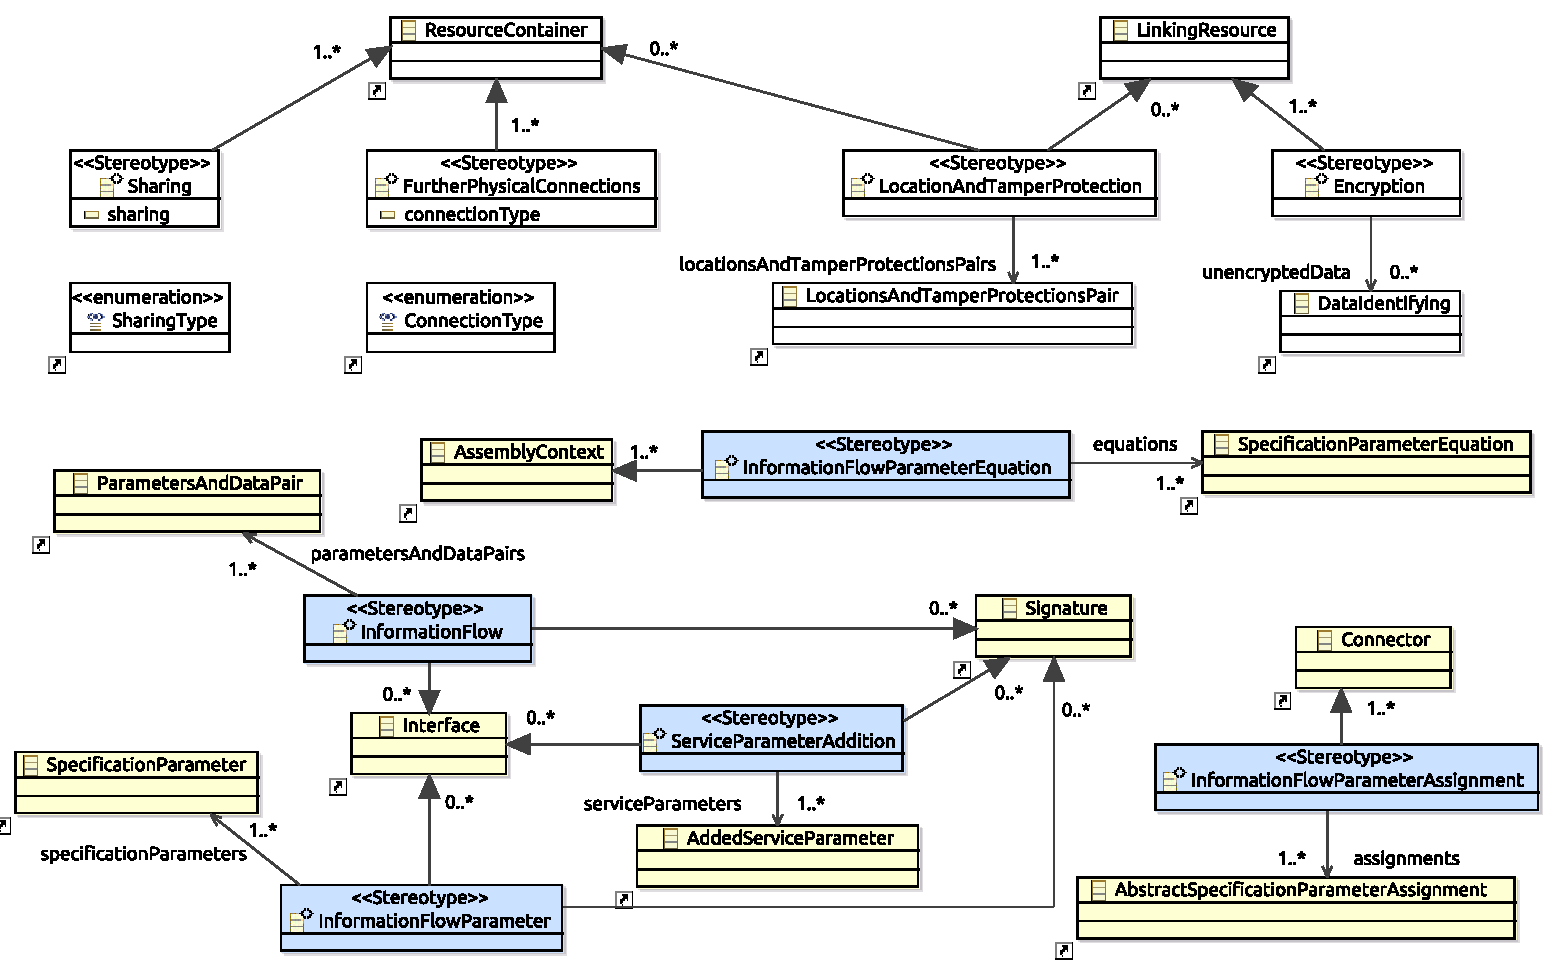
\includegraphics[width=0.9\textwidth]{images/confidentiality_profile.pdf}
	%\includegraphics[width=0.9\textwidth]{images/WordCloud.png}
	\vspace{0.05\textheight}
	\column{.25\textwidth}
	\texttt{\footnotesize dataSet(2).\\
		parametersAndDataPair(8).\\
		parameterSources(8,[return]).\\
		dataTargets(8,[5,6,7,4]).}
	\column{.25\textwidth}
	\texttt{\tiny isInSecureWithRespectTo(guest)\\
+- accessibleParameters(guest,return(getId))\\
| +- linksDataAccessibleBy(guest,wireless)\\
| | +- linkAccessibleBy(guest,wireless)\\
| | | +- linkLocation(wireless)
| | | ‘- locationsAccessibleBy(guest)}
\end{columns}
\begin{columns}\centering
	\column{.25\textwidth}
	\centering
	\textbf{Palladio Component Model}
	\vspace{0.05\textheight}
	\column{.25\textwidth}
	\centering
	\textbf{Confidentiality Model}
	\column{.25\textwidth}
	\centering
	\textbf{Prolog Prädikate}
	\column{.25\textwidth}
	\centering
	\textbf{Analyse Ergebnis}
\end{columns}
\begin{columns}\centering
\column{.1\textwidth}
\column{.25\textwidth}
\centering
$\longrightarrow$ \\
Confidentiality4CBSE
\column{.25\textwidth}
\centering
$\longrightarrow $\\
PCM2Prolog
\column{.25\textwidth}
\centering
$\longrightarrow$ \\
\textcolor{gray}{Haskalladio}
\column{.1\textwidth}
\end{columns}
\end{frame}	


\begin{frame}{Vertraulichkeitsmodellierung}{Datenfluss}
	\begin{itemize}
		\item Daten werden in DataSets getrennt
		\item Information Flow ordnet Datenfluss an Operationen DataSets zu
		\begin{itemize}
			\item Parameter
			\item Rückgabewert
			\item Aufruf der Funktion
			\item Größe von Paramtern
		\end{itemize}
	\end{itemize}

\end{frame}	
\begin{frame}{Vertraulichkeitsmodellierung}{Ressourcen}
ResourceContainer:
	\begin{itemize}
		\item Zusätzlich mögliche Verbindungen
		\item geteilt Laufzeitumgebung
	\end{itemize}
LinkingResource:
	\begin{itemize}
		\item Welche Daten werden unverschüsselt übertragen?
	\end{itemize}
ResourceContainer + LinkingResource:
\begin{itemize}
	\item Welche Maßnahmen (Tamper-Protections) wurden getroffen um Ressourcen zu schützen
\end{itemize}
\end{frame}	
\begin{frame}{Vertraulichkeitsmodellierung}{Angreifer}
	\begin{itemize}
		\item Welche DataSet dürfen bekannt sein?
		\item Welche Tamper-Protections kann/will der Angreifer umgehen?
		\item Wo hat der Angreifer Zugriff?
	\end{itemize}
\end{frame}	


\section{Modell}
\begin{frame}{Bisheriges Modell}{Profil-Mechanismus}
\begin{columns}
	\column{0.55\textwidth}
Confidentiality Modell: 
\begin{itemize}
	\item Definiert Klassen zum Modellieren von DataSet, Maßnahmen, Angreifer, ...
\end{itemize}
Confidentiality-Profil:
\begin{itemize}
	\item Zusammenfassung von mehreren Stereotypen
	\item Stereotyp erweitert eine oder mehrere PCM Klassen
	\item Stereotyp hat Referenzen zu Elementen aus dem Confideniality-Modell
\end{itemize}%
$\rightarrow$ soll entfernt werden
\column{0.35\textwidth}\centering
\includegraphics[width=\textwidth]{images/stereotype.pdf}
\end{columns}
\end{frame}	

\begin{frame}{Entfernen Profil-Mechanismus}
	\begin{columns}
		\column{0.4\textwidth}\centering
	\includegraphics[width=\textwidth]{images/stereotype.pdf}
	\column{0.1\textwidth}\centering
	$\rightarrow$
	\column{0.5\textwidth}\centering
	\includegraphics[width=\textwidth]{images/location_tamperprotection.pdf}
	\end{columns}
\end{frame}
\begin{frame}{Entfernen Profil-Mechanismus}
	\begin{columns}
		\column{0.5\textwidth}\centering
		\includegraphics[width=\textwidth]{images/resoucrecontainer_linkingresouce.pdf}
		\column{0.1\textwidth}\centering
		$\rightarrow$
		\column{0.3\textwidth}\centering
		\includegraphics[width=\textwidth]{images/resources_container.pdf}
	\end{columns}
\end{frame}

\begin{frame}{Bisheriges Modell}{Information Modellierung}
		\begin{columns}
		\column{0.55\textwidth}
		\begin{itemize}
			\item Zuordnung von DataSets und Datenflüssen an Operationen erfolgt über Strings\\
			$\rightarrow$ implizite Referenz\\
			$\rightarrow$ Verwechslungsgefahr bei gleichnamigen Parametern
		\end{itemize}
		$\rightarrow$ soll explizit modelliert werden
		\column{0.35\textwidth}
		\begin{center}
			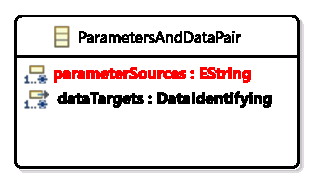
\includegraphics[width=0.9\textwidth]{images/ParameterAndDataPair.pdf}
		\end{center}
		\vspace{0.02\textheight}
		\texttt{parameterSource = ''resquestData''}\\
		\texttt{parameterSource = ''$\backslash$return''}\\
		\texttt{parameterSource = ''$\backslash$call''}\\
		\texttt{parameterSource = ''*''}\\
		\texttt{parameterSource = ''sizeof(*)''}
	\end{columns}	
\end{frame}

\begin{frame}{Informations-Modellierung}
	\begin{columns}
		\column{0.25\textwidth}\centering
		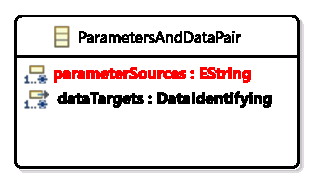
\includegraphics[width=\textwidth]{images/ParameterAndDataPair.pdf}
		\column{0.1\textwidth}\centering
		$\rightarrow$
		\column{0.6\textwidth}\centering
		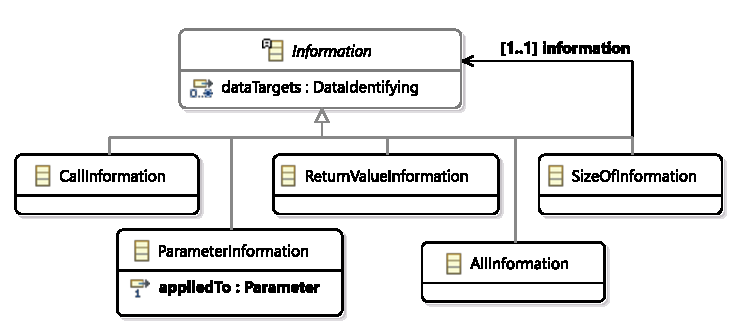
\includegraphics[width=\textwidth]{images/information.pdf}
	\end{columns}
\end{frame}
\section{PCM2Prolog}
\begin{frame}{PCM2Prolog}
	\begin{itemize}
		\item xTend
		\item Reflective-API wird verwendet um Entitäten auf Prolog Prädikate abzubilden
		\item Filter bestimmt relevante Entitäten und Referenzen
	\end{itemize}
\vspace{0.05\textheight}
	\begin{columns}
		\column{0.6\textwidth}\centering
		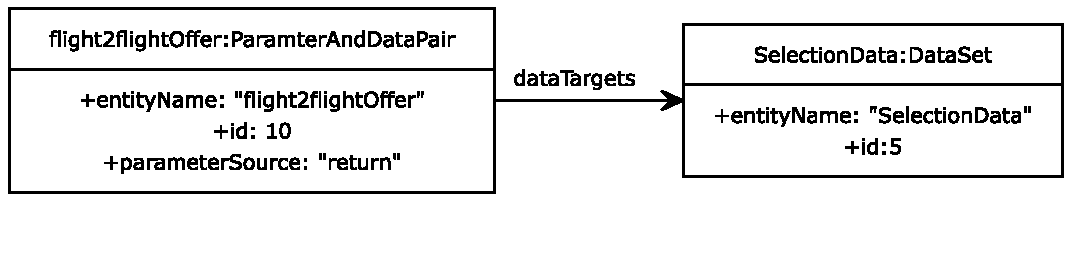
\includegraphics[width=0.9\textwidth]{images/pcm2prologUml.pdf}
		\column{0.1\textwidth}\centering
		$\rightarrow$
		\column{0.35\textwidth}
		\texttt{parametersAndDataPair(10).\\
			parameterSources(10,[return]).\\
			dataTargets(10,[5]).\\ \vspace{0.05\textheight}
			dataSet(5).}
	\end{columns}
\end{frame}	
\begin{frame}{Anpassungen PCM2Prolog}
	\begin{itemize}
		\item Dispatch-Methoden für Entitäten die nicht automatisch generiert werden können \\ \vspace{0.05\textheight}
		\texttt{def dispatch String generateDeeplyCorrectly(EObject e) $\{$
				return super.generateDeeply(e)
		$\}$}\\
		\texttt{def dispatch String generateDeeplyCorrectly(AbstractResourceProtection rp) $\{...\}$} \\ \vspace{0.05\textheight}
		\item Ursprüngliche Stereotypen Referenzen müssen umgedreht werden
		\begin{itemize}
			\item Map<EObject,Set<String> > für jeden Stereotyp der auf PCM Komponenten angewandt werden kann
			\item Beim Verarbeiten der neuen Klassen wird deren ID dem zur PCM Komponente gehörenden Set hinzugefügt
			\item Nach dem alle Entitäten verarbeiten wurden $\rightarrow$ erzeuge Prädikate aus den Map Elementen
		\end{itemize}
	\end{itemize}
\end{frame}
\section{Evaluierung}
\begin{frame}{Evaluierung}
	Modellierung der Beispiel Projekte \texttt{cloudscenario-minimized}\footnote{https://github.com/KASTEL-SCBS/Examples4SCBS/tree/master/bundles/edu.kit.kastel.scbs.cloudscenario-minimized} und \texttt{iflowexample}\footnote{https://github.com/KASTEL-SCBS/Examples4SCBS/tree/master/bundles/edu.kit.kastel.scbs.iflowexample} 5mit dem neuen Modell:
	\begin{itemize}
		\item Gleiche IDs verwenden
	\end{itemize}
	Automatischer Vergleich des Prolog Codes:
	\begin{itemize}
		\item Prolog Datei vorverarbeiten:
		\begin{itemize}
			\item Listen innerhalb Prolog Prädikate sortieren:
			\texttt{prädikat(5, [''b'',''c'',''a'']).} wird zu \texttt{prädikat(5, [''a'',''b'',''c'']).}
			\item Zeilen der Datei sortieren
			\item Leerzeilen entfernen
		\end{itemize}
		\item Ausgabe mit \texttt{diff} vergleichen
	\end{itemize}
 $\rightarrow$ für diese Projekte möglich, aber nicht für alle möglichen Instanzen des ursprünglichen Modells
\end{frame}

\appendix
\beginbackup
 %% ----------------------------------------
%% | /Test-Folie mit definierten Farben |
%% ----------------------------------------
\backupend

\end{document}